\documentclass{article}
\usepackage[left=3cm, right=3cm, top=0cm]{geometry}
\usepackage{amsmath}
\usepackage{graphicx}
\usepackage{tikz}

\setlength{\parindent}{0pt}
\begin{document}
\title{CS112 LBA}
\author{Jacob Puthipiroj}
\date{}
\maketitle

Hello Vivian, Katka, as per our meeting on Tuesday, I'd like to go into further detail about the matching algorithm I proposed.

\section*{Executive Summary}
Instead of relying solely on human judgment for the matching of startups to investors on Investors' Day, Betahaus can use a simple matching algorithm to compute the level of 'fit' of each startup to each investor, and order each startup by said fitness score. This a simple algorithm for which data can easily be implemented in currently existing customer-facing interfaces, such as EventBrite signup sheets. Having an algorithmically sorted list for each startup will significantly reduce the amount of human hours to be spent on this task.

\section*{Problem Framing}
Betahaus, as a community of entrepreneurs, often organizes multiple events year-round in order to grow the startup ecosystem in Berlin. One of the largest of these events is the Investors' Day, held annually in November. In recent years, the number of attendees has grown exponentially; the attendance in 2018 is guaranteed to include at least 300 startup representatives and 30 investors. With it being impossible for every investor to spend time individually with each startup, each investor aims to spend time only with startups that are most relevant to their own interests. To date, this has been done manually - Betahaus staff will spend hours finding attendees in the startup list which they believe have the closest matches to the investor, based on their own understanding of investor preferences. However, this process can be significantly automated by way of a matching algorithm.\footnote{\#utility: For all stakeholders involved, the algorithm was a boon. Investors could be supplied not only with handful of startups selected to match them on, but an entire customized list of all startup attendees ranked in order of relevancy. For Betahaus, the amount of time spent on tedious tasks was significantly reduced. For investors, they were paired with investors who were already interested in what they had to present.}
 
\section*{Data Required}
The matching algorithm requires relatively small amounts of data that can be easily (and is currently) gathered in the EventBrite signup pages. This includes, from the startups:
\begin{itemize}
\itemsep-0.3em 
	\item Field of interest (The question is posed as a 'check all that apply' decision)
	\item Necessity of investors (A binary yes/no variable)
	\item Startup stage (An categorical variable of Idea/Prototype/Product Launched)
	\item Funding round (An ordinal variable of Pre-seed/Seed/Series A and beyond)
	\item Location of the startup (A City name that is looked up for its coordinates on Google Maps)
\end{itemize}
Furthermore, the following preferences are required from the investors:
\begin{itemize}
\itemsep-0.3em 
	\item Field of interest (The question is posed as a 'check all that apply')
	\item Startup stage preference ('Check all that apply' for Idea/Prototype/Product Launched)
	\item Funding Round preference ('Check all that apply' for Pre-Seed/Seed/Series A and beyond)
	\item Location preferences (If there are preference, input City name and the radius for which to consider startups, if none, leave blank).
\end{itemize}
\newgeometry{left=3cm,right = 3cm,}

\section*{Methodology}
\begin{enumerate}
\itemsep-0.3em 
\item Start with the first investor.
\item Filter startups on 'Startup stage' and 'Funding round' variables. \begin{itemize} 
\itemsep-0.3em 
\item For example, if the investor does not want to consider startups in the idea stage or in the Pre-Seed stage, then temporarily remove them from the list of startups   \end{itemize}
\item Create a matrix of matches: \begin{itemize} \itemsep-0.3em 
\item The columns indicate the investors' interests, while rows indicate startups' field of interests. 
\item For example, for an investor interested in 'SaaS', 'Enterprise', and 'Developer Tools', and with Startup A interested in 'SaaS', 'Enterprise' and 'Smart Mobility', and with Startup B interested in 'Smart Mobility', 'FashionTech' and 'SaaS', the matrix is\\

\begin{tabular}{llll}
\hline
\multicolumn{1}{|l|}{Investor Fields of Interest} & \multicolumn{1}{l|}{SaaS} & \multicolumn{1}{l|}{Enterprise} & \multicolumn{1}{l|}{Developer Tools} \\ \hline
\multicolumn{1}{|l|}{Startup A}                   & \multicolumn{1}{l|}{1}    & \multicolumn{1}{l|}{1}          & \multicolumn{1}{l|}{0}               \\ \hline
\multicolumn{1}{|l|}{Startup B}                   & \multicolumn{1}{l|}{1}    & \multicolumn{1}{l|}{0}          & \multicolumn{1}{l|}{0}               \\ \hline
                                                  &                           &                                 &                                     
\end{tabular}
\item 1 indicates a shared interest in a field, while 0 indicates no shared interest.
\item By looking at the matrix, we can see that Startup A is at least as relevant to the investor than Startup B is, because it shares all of Startup B's interests, plus one more. All of the startups' other interests are ignored.
 \end{itemize}
\item Scale the matrix. \begin{itemize} \itemsep-0.3em 
\item This is done by dividing each cell in the matrix by the \textit{standard deviation} for that column. However, if the standard deviation for that column is 0, then set the entire column to 0.
\item The reasoning behind this is that the rarity of each interest should be taken into account. In the above example, the fact that both Startups are interested in SaaS makes the column relatively unimportant. Similarly, the fact that neither is interested in Developer Tools makes that column unimportant. The only important column here, is actually `Enterprise', since there is a mix of both 1s and 0s. Standard deviation takes this rarity of the columns into account.


\item In the above example, the matrix obtained would be: \\ 

\begin{tabular}{llll}
\hline
\multicolumn{1}{|l|}{Investor Fields of Interest} & \multicolumn{1}{l|}{Saas} & \multicolumn{1}{l|}{Entreprise} & \multicolumn{1}{l|}{Developer Tools} \\ \hline
\multicolumn{1}{|l|}{Startup A}                   & \multicolumn{1}{l|}{0}    & \multicolumn{1}{l|}{0.7071}     & \multicolumn{1}{l|}{0}               \\ \hline
\multicolumn{1}{|l|}{Startup B}                   & \multicolumn{1}{l|}{0}    & \multicolumn{1}{l|}{0}          & \multicolumn{1}{l|}{0}               \\ \hline
                                                  &                           &                                 &                                     
\end{tabular}
 \end{itemize}
\item Add up the sums of each column to obtain the final score, and sort by said score \begin{itemize}
\itemsep-0.3em \item In the example, this would be 0.7071 for Startup A, and 0 for Startup B.
\item Hence, Startup A should be ranked higher than Startup B. 
\end{itemize}


\item Repeat steps 2-5 for each new investor.\footnote{\#audience: In order for the investors to know what I am talking about, I try to make the explanation as clear as possible, I try to use examples that are as simple as possible, involving only 2 startups and 3 investor fields, as well as providing extensive reasoning.}
\end{enumerate}


\section*{Conclusion and Next Steps}
With an exponentially growing number of attendees to Betahaus events, it is quickly becoming infeasible to rely solely on manpower to ensure satisfaction of investors when it comes to presenting portfolio startups. By using an algorithm that sorts startups by relevancy, Betahaus staff can more effectively choose matches for each investor.\footnote{\#cognitivepersuasion: This was simple but effective. The idea that they could save tons of time (a staff member reported spending over 7 hours for the previous' years events, plus time spent on similar events) for a rapidly growing problem was so appealing that I only had to present the product for them to jump on board. I have already implemented this algorithm over the past week.}\footnote{\#professionalism: I formatted the work in a clear and concise manner.}

	
\begin{figure*}[h]
\center
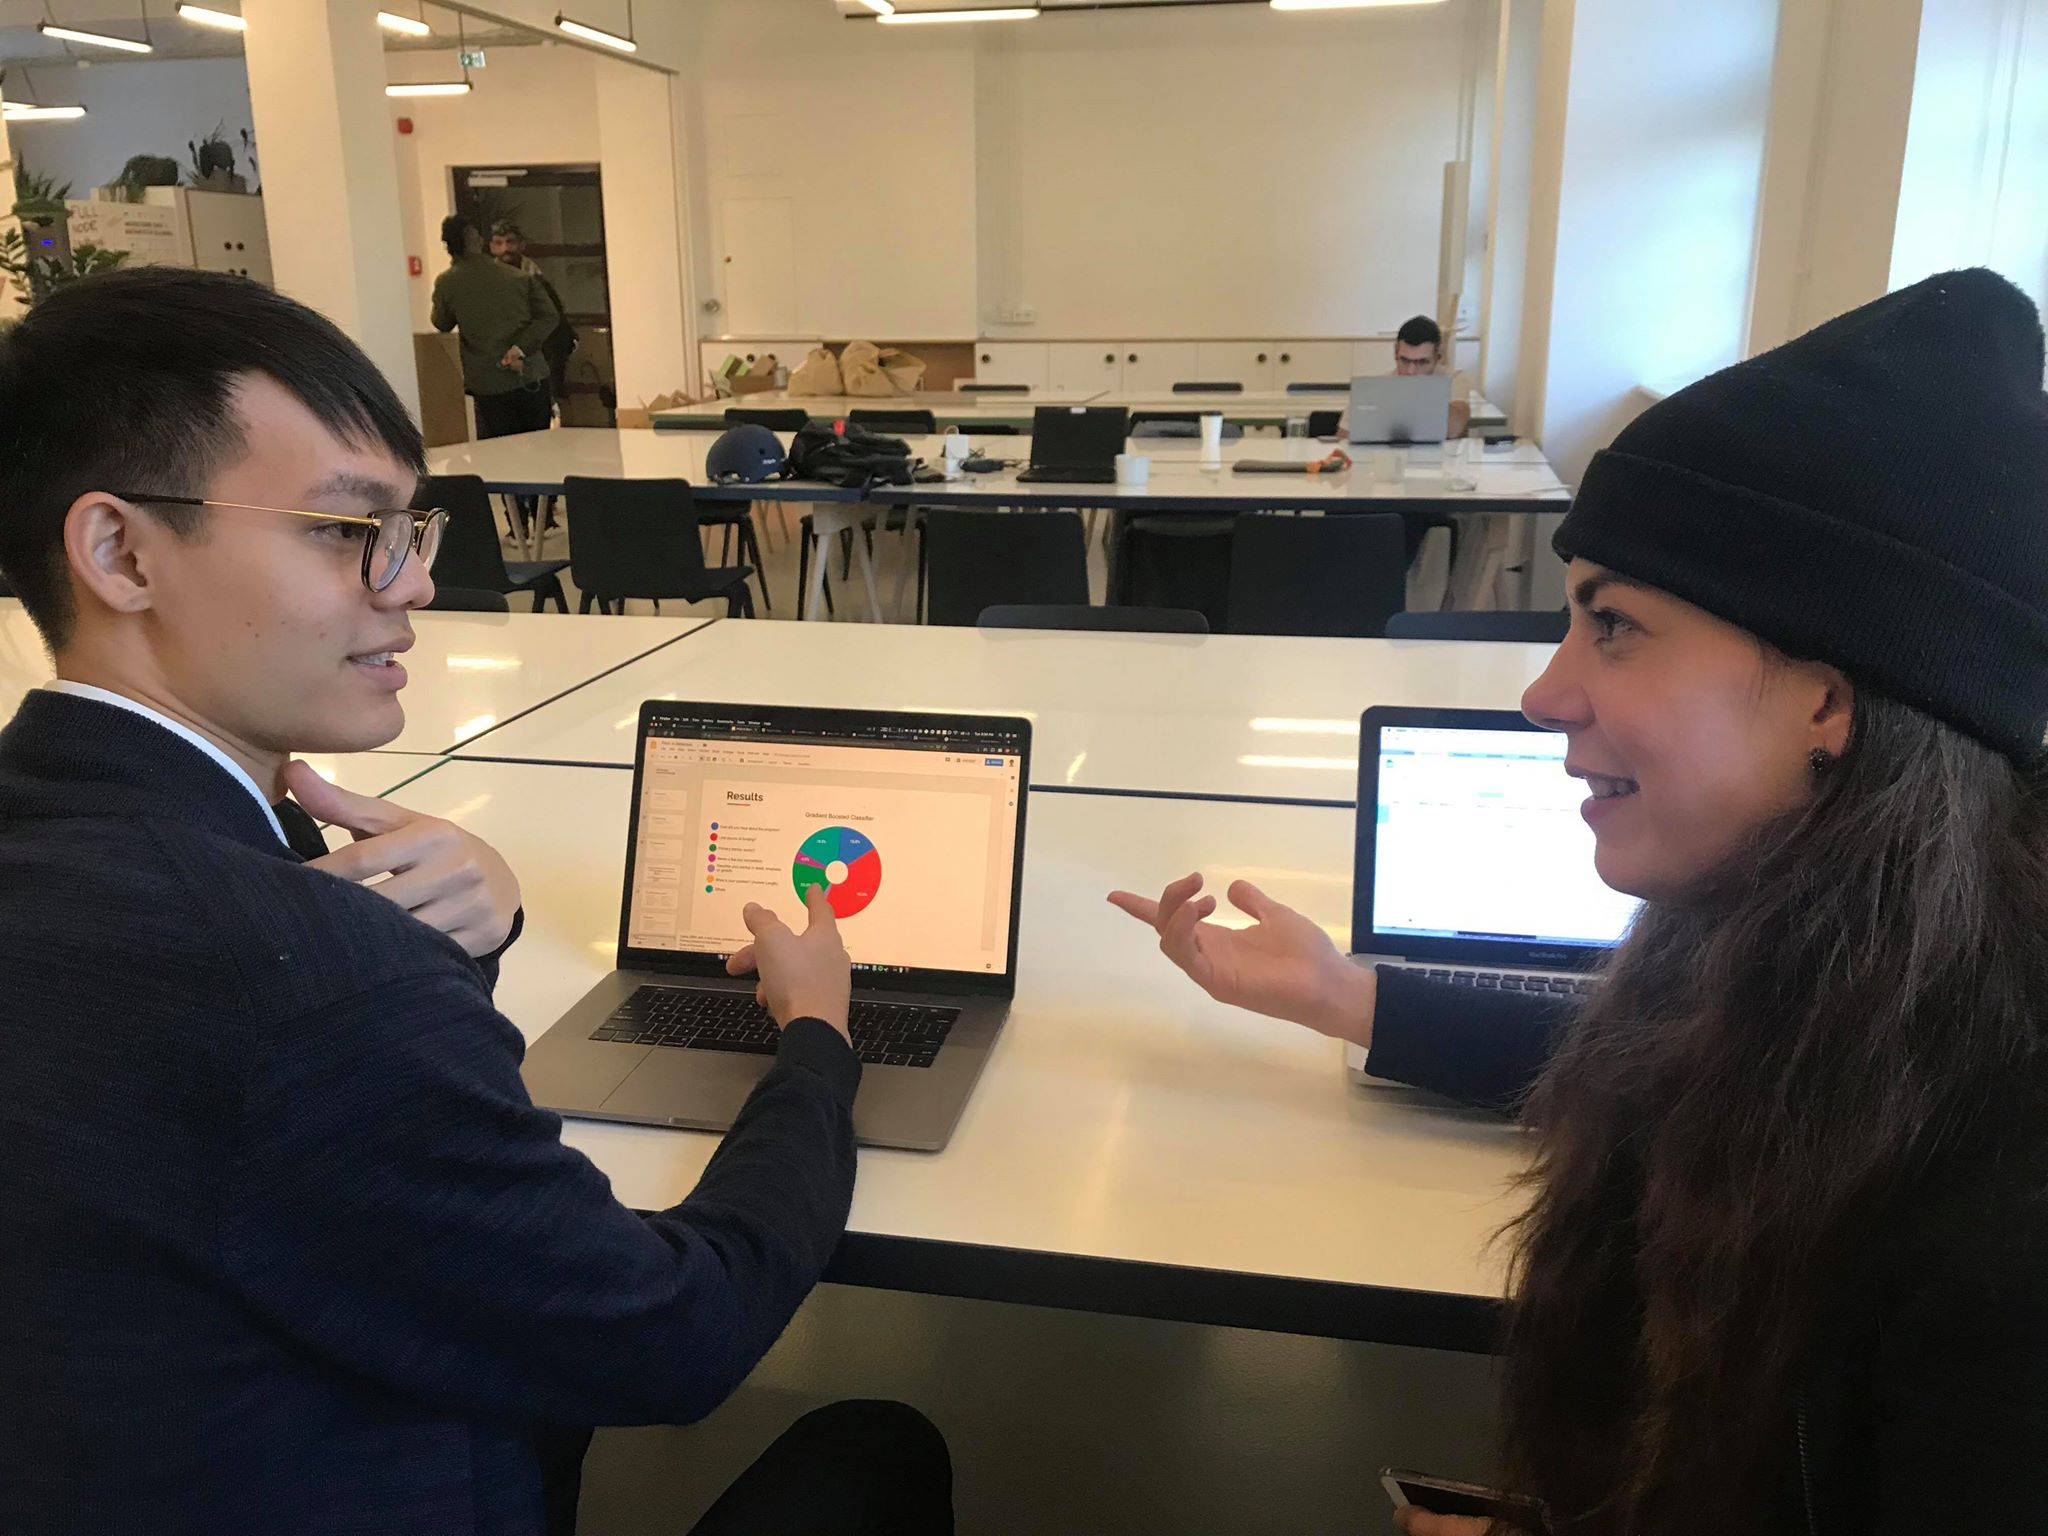
\includegraphics[scale = 0.2]{katka.jpg}
\caption{A meeting with Katka on November $6^{\textrm{th}}$, 2018.}
\end{figure*}

\section*{Technical Appendix}
All code for the assignment is 





	
\end{document}
